\documentclass[11pt, a4paper, twoside]{montblanc}

\usepackage[utf8]{inputenc}
\usepackage{hyperref}
\usepackage{listings}
\usepackage{color}
\usepackage{xspace}

\newcommand{\productname}[1]{\textsc{#1}}
%\newcommand{\latin}[1]{\textit{#1}}

\newcommand{\Specfem}{\productname{Specfem 3D}\xspace}
\newcommand{\Cuda}{\productname{Cuda}\xspace}
%\newcommand{\eg}{\latin{e.g.,}\xspace}
\newcommand{\OCL}{\productname{OpenCL}\xspace}
\newcommand{\code}[1]{\texttt{#1}}

%\newcommand{\etc}[1]{\latin{etc}}

%\usepackage{lineno}
%\modulolinenumbers[5]
%\linenumbers

\lstdefinestyle{customc}{
  language=C,
  basicstyle=\scriptsize,
  backgroundcolor=\color{white},
  frame=single,
  captionpos=b,
  morekeywords={int64_t, int32_t}
}

\lstdefinestyle{customgputrace}{
  language=C,
  basicstyle=\scriptsize,
  backgroundcolor=\color{white},
  frame=single,
  captionpos=b,
  morekeywords={New, kernel, buffer, Mb, READ_WRITE, Buffer, written,
    b, at, out}
}

\lstdefinestyle{customcl}{
  language=C,
  basicstyle=\scriptsize,
  backgroundcolor=\color{white},
  frame=single,
  captionpos=b,
  morekeywords={__global, __local, global, local, __kernel, kernel, short,
uchar, uchar16, int16, short16}
}

\lstdefinestyle{BOAST}{
  language=Ruby, 
  basicstyle=\scriptsize, 
  backgroundcolor=\color{white}, 
  frame=single, 
  captionpos=b,
  morekeywords={BOAST, pr, decl, opn, close}
}

\lstdefinestyle{customf}{
  language=FORTRAN,
  basicstyle=\scriptsize,
  backgroundcolor=\color{white},
  frame=single,
  captionpos=b
}

\lstdefinestyle{custombash}{
  language=Bash,
  basicstyle=\scriptsize,
  backgroundcolor=\color{white},
  frame=single,
  captionpos=b
}


\usepackage{url}


\bibliographystyle{plain}
\begin{document}
\devnum{5.5}
\title{BOAST: a Metaprogramming Framework to Produce Portable and Efficient Computing Kernels for HPC Applications}
\version{0.5}
\deadline{18}
\level{RE}
\nature{Report}
\coordinator{CNRS}
\contributors{Thierry Deutsch (CEA), Luigi Genovese (CEA), Jean-François Méhaut (UJF), Kevin Pouget (CNRS), Brice Videau (CNRS)}
\reviewers{Olivier Aumage (INRIA), Frédéric Desprez (INRIA), Harald Servat (BSC)}
\keywords{BOAST, Deliverable}

\maketitle

\begin{changelog}
\change{0.1}{Initial version of the deliverable}
\change{0.2}{First version sent to reviewers}
\change{0.3}{With corrections from reviewers}
\change{0.4}{Additional corrections from reviewers}
\end{changelog}

\frontmatter

\begin{executive}
This document describes BOAST, a metaprogramming framework to produce portable
and efficient computing kernels for HPC application. BOAST offers an embedded
domain specific language to describe the kernels and their possible
optimization. BOAST also supplies a complete run-time to compile, run, benchmark,
and check the validity of the generated kernels. BOAST is being used in two
flagship HPC applications BigDFT and SPECFEM3D, to improve performance
portability of those codes.
\end{executive}

\section{Introduction}

Porting and tuning HPC applications to new platforms is tedious and costly in
terms of human resources. Nonetheless, it is a very important aspect of the
Mont-Blanc project. Indeed, for the project, more than ten applications were
selected to be ported and optimized for the prototype platform.

Unfortunately, portability efforts are often lost when migrating to a new
architecture. Worse, code may lose maintainability because several versions of
some functionalities coexist, usually with a lot of duplication.

Thus productivity of porting and tuning efforts is low as a huge fraction of
those developments are never used after the platform they were intended for is
decommissioned.

Genericity of HPC codes is often limited. One of the reason is that producing
generic code in Fortran 90/95 is difficult as the language does not really fit
for it. Sometimes, adding genericity degrades performance as optimization
opportunities that come from over-specification are lost.

Functionality of HPC codes is tied to the previous point. Without genericity,
adding new functionalities can be quite costly.

\section{Background and Motivation}

  \subsection{Scientific Computing Applications}

Scientific Computing Applications are usually developed by physicist, chemist or
meteorologist. Those codes are usually written in Fortran for historical and
performance reasons. Codes can be quite huge (several thousands lines of code [LOC])
with lots of functionalities. Nonetheless, they are usually based on computing
kernels.  Computing kernels are resource intensive and well-defined parts of a
program that usually work on precisely defined data. Those kernels represent the most
time-consuming part of an HPC application, and consequently, they are the prime target for
optimization.

Those applications are often developed by several individuals. Sometimes, some
of those developers only work a few months on the application. Maintaining
optimized code written by someone else is quite a challenge. Several languages
and programming paradigms can also be used in a project and thus the maintainer
must be knowledgeable in several areas of expertise. Portability problems can
also be caused by the availability of an optimizing compiler for a specific
language and architecture. C compilers are usually the first available while
Fortran may sometimes arrive later.

In Section~\ref{use_cases} we will present two HPC applications that we used
as use cases: SPECFEM3D and BigDFT. They are both based on computing
kernels and were selected as candidate applications in the Mont-Blanc project.

  \subsection{How Should Computing Kernels be Written?}

The problematic here is to obtain computing kernels that present good
performances on the architectures encountered by the application while still
being portable after the optimization process took place. Indeed the
application might encounter one of the many architectures that can be found in
HPC. Investing manpower to optimize the application for a new architecture is
reasonable, suffering hindrance from previous optimization work is not. Thus
optimizations have to be as orthogonal as possible from one another so as to be
easily activated and deactivated.

If this paradigm is followed by developers then they will rapidly be confronted
with a huge optimization space to search. They will need to be able to test
easily the performance impact of the chosen optimizations without running the
full application. The same reasoning implies that kernels should be tested for
non regression without running the full application.

What we want is computing kernels that are written:
\begin{itemize}
\item in a \emph{portable} manner,
\item in a way that raises developer \emph{productivity},
\item and, present good \emph{performance}.
\end{itemize}



  \subsection{Evolution of HPC Architectures}

Evolution of HPC Architectures is rapid and also diverse: in the last 5
years no less than 6 architectures have been number one in the Top500:
\begin{itemize}
\item Intel Processor + Xeon Phi (Tianhe-2)
\item AMD Processor + NVIDIA GPU (Titan)
\item IBM BlueGene/Q (Sequoia)
\item Fujitsu SPARC64 (K computer)
\item Intel Processor + NVIDIA GPU (Tianhe-1)
\item AMD Processor (Jaguar)
\end{itemize}
Being able to efficiently use those architectures on such a small
time-frame is challenging.

The race to exascale is not going to simplify the environment. All of the above
architectures can be considered. Network architectures also can be very
diverse.  For instance European FP7 project DEEP considers using Accelerators
(XEON Phi) while the European FP7 project Mont-Blanc considers using low-power
embedded processor with integrated GPU.

Running existing applications on those new architectures is an open research
subject as well as an ongoing porting effort.  Thus, those projects have work
packages dedicated to applications. Those work packages are dedicated to porting
and optimizing Scientific applications on those new architectures. In the DEEP
project six applications were selected for porting and optimizing, eleven were
selected in the Mont-Blanc project.

\section{Motivating Example: OpenCL Laplace}
\label{sec:laplace}

During one of the Mont-Blanc face to face meeting a talk on OpenCL optimization
on the Mali GPU was given. One of the case study was a Laplace filter on the
GPU~\cite{opencl_arm_training}.

This is a good example of an algorithm that is simple in its formulation but
can be complex to optimize because many different optimizations are available
and can be combined together. The correct combination of optimizations will
depend on the targeted architecture.

\subsection{The Laplace Filter}

Listing~\ref{lst:laplace_c_filter} shows a simple implementation of the Laplace
filter in C99. For clarity, boundary conditions have been omitted.

\lstset{style=customc,
        caption={Laplace C99 Filter},
        breaklines=true,
        breakautoindent=false,
        label={lst:laplace_c_filter}}
\begin{lstlisting}
void laplace(const int width,
             const int height,
             const unsigned char src[height][width][3],
                   unsigned char dst[height][width][3]){
  for (int j = 1; j < height-1; j++) {
    for (int i = 1; i < width-1; i++) {
      for (int c = 0; c < 3; c++) {
        int tmp = -src[j-1][i-1][c] -   src[j-1][i][c] - src[j-1][i+1][c]\
                 - src[j  ][i-1][c] + 9*src[j  ][i][c] - src[j  ][i+1][c]\
                 - src[j+1][i-1][c] -   src[j+1][i][c] - src[j+1][i+1][c];
        dst[j][i][c] = (tmp < 0 ? 0 : (tmp > 255 ? 255 : tmp));
      }
    }
  }
}
\end{lstlisting}

A naive implementation in OpenCL is proposed in
Listing~\ref{lst:laplace_opencl_filter}. Each work item processes one pixel of
the resulting image.

\lstset{style=customcl,
        caption={Laplace OpenCL Filter},
        breaklines=true,
        breakautoindent=false,
        label={lst:laplace_opencl_filter}}
\begin{lstlisting}
kernel laplace(const int width,
               const int height,
               global const uchar *src,
               global       uchar *dst){
  int i = get_global_id(0);
  int j = get_global_id(1);
  for (int c = 0; c < 3; c++) {
    int tmp = -src[3*width*(j-1) + 3*(i-1) + c]\
             - src[3*width*(j-1) + 3*(i  ) + c]\
             - src[3*width*(j-1) + 3*(i+1) + c]\
             - src[3*width*(j  ) + 3*(i-1) + c]\
           + 9*src[3*width*(j  ) + 3*(i  ) + c]\
             - src[3*width*(j  ) + 3*(i+1) + c]\
             - src[3*width*(j+1) + 3*(i-1) + c]\
             - src[3*width*(j+1) + 3*(i  ) + c]\
             - src[3*width*(j+1) + 3*(i+1) + c];
    dst[3*width*j + 3*i + c] = clamp(tmp, 0, 255);
  }
}
\end{lstlisting}



\subsection{Possible Optimizations of the OpenCL Version}

Several optimizations were proposed and successively applied to the previous
implementation.

\paragraph{Vectorization}
The first proposed optimization involves computing five pixels instead of one using the
vectors available to the Mali architecture. The vectors have to reside in memory to
ensure an efficient execution. Using vectors of 16 elements, 15 useful components
are simultaneously loaded and can be used in computation. This optimization
yields speedups between 1.5 and 6 depending on the image size.

\lstset{style=customcl,
        caption={Laplace OpenCL Filter Vectorized},
        breaklines=true,
        breakautoindent=false,
        label={lst:laplace_opencl_filter_vector}}
\begin{lstlisting}
kernel laplace(const int width,
               const int height,
               global const uchar *src,
               global       uchar *dst){
  int i = get_global_id(0);
  int j = get_global_id(1);

  uchar16 v11_ = vload16( 0, src + 3*width*(j-1) + 3*5*i - 3 );
  uchar16 v12_ = vload16( 0, src + 3*width*(j-1) + 3*5*i     );
  uchar16 v13_ = vload16( 0, src + 3*width*(j-1) + 3*5*i + 3 );
  uchar16 v21_ = vload16( 0, src + 3*width*(j  ) + 3*5*i - 3 );
  uchar16 v22_ = vload16( 0, src + 3*width*(j  ) + 3*5*i     );
  uchar16 v23_ = vload16( 0, src + 3*width*(j  ) + 3*5*i + 3 );
  uchar16 v31_ = vload16( 0, src + 3*width*(j+1) + 3*5*i - 3 );
  uchar16 v32_ = vload16( 0, src + 3*width*(j+1) + 3*5*i     );
  uchar16 v33_ = vload16( 0, src + 3*width*(j+1) + 3*5*i + 3 );

  int16 v11 = convert_int16(v11_);
  int16 v12 = convert_int16(v12_);
  int16 v13 = convert_int16(v13_);
  int16 v21 = convert_int16(v21_);
  int16 v22 = convert_int16(v22_);
  int16 v23 = convert_int16(v23_);
  int16 v31 = convert_int16(v31_);
  int16 v32 = convert_int16(v32_);
  int16 v33 = convert_int16(v33_);

  int16 res = v22 * (int)9 - v11 - v12 - v13 - v21 - v23 - v31 - v32 - v33;
        res = clamp(res, (int16)0, (int16)255);
  uchar res_ = convert_uchar16(res);

  vstore8(res_.s01234567, 0, dst + 3*width*j + 3*5*i);
  vstore8(res_.s89ab,     0, dst + 3*width*j + 3*5*i + 8);
  vstore8(res_.scd,       0, dst + 3*width*j + 3*5*i + 12);
  dst[3*width*j + 3*5*i + 14] = res_.se;
}
\end{lstlisting}

\paragraph{Synthesizing Loads} It is possible to reduce the number of loads
since the vectors are overlapping.
Listing~\ref{lst:laplace_opencl_filter_vector_synth} shows how the vectors are
loaded in this case. This optimization yields marginal improvements.

\lstset{style=customcl,
        caption={Laplace OpenCL Filter Vectorized with Synthesized Loads},
        breaklines=true,
        breakautoindent=false,
        label={lst:laplace_opencl_filter_vector_synth}}
\begin{lstlisting}
  uchar16 v11_ = vload16( 0, src + 3*width*(j-1) + 3*5*i - 3 );
  uchar16 v13_ = vload16( 0, src + 3*width*(j-1) + 3*5*i + 3 );
  uchar16 v12_ = uchar16( v11_.s3456789a, v13_.s56789abc );
  uchar16 v21_ = vload16( 0, src + 3*width*(j  ) + 3*5*i - 3 );
  uchar16 v23_ = vload16( 0, src + 3*width*(j  ) + 3*5*i + 3 );
  uchar16 v22_ = uchar16( v21_.s3456789a, v23_.s56789abc );
  uchar16 v31_ = vload16( 0, src + 3*width*(j+1) + 3*5*i - 3 );
  uchar16 v33_ = vload16( 0, src + 3*width*(j+1) + 3*5*i + 3 );
  uchar16 v32_ = uchar16( v31_.s3456789a, v33_.s56789abc );
\end{lstlisting}

\paragraph{Temporary Variables Size} Using \textit{int} to store intermediary
results is unnecessary. Listing~\ref{lst:laplace_opencl_filter_short} show how
the code is modified to use smaller types. This yields a speedup of 1.3 for most
image sizes.

\lstset{style=customcl,
        caption={Laplace OpenCL Filter Vectorized Using \textit{short}},
        breaklines=true,
        breakautoindent=false,
        label={lst:laplace_opencl_filter_short}}
\begin{lstlisting}
  short16 v11 = convert_short16(v11_);
  short16 v12 = convert_short16(v12_);
  short16 v13 = convert_short16(v13_);
  short16 v21 = convert_short16(v21_);
  short16 v22 = convert_short16(v22_);
  short16 v23 = convert_short16(v23_);
  short16 v31 = convert_short16(v31_);
  short16 v32 = convert_short16(v32_);
  short16 v33 = convert_short16(v33_);

  short16 res = v22 * (short)9 - v11 - v12 - v13 - v21 - v23 - v31 - v32 - v33;
          res = clamp(res, (short16)0, (short16)255);
\end{lstlisting}

\paragraph{More Optimizations} Several other optimizations can be attempted at
this point. For instance reducing or increasing the number of pixels each work
item is processing. They can yield improved performance in some cases, especially
when avoiding memory alignment problems. These optimizations will not be shown
here but can be found in~\cite{opencl_arm_training}.

\subsection{Improving the Methodology}

The process described in the previous Subsection is quite tedious and requires
some intimate knowledge of the target architecture. The results are impressive,
as speedups of almost 10 are observed compared to the naive OpenCL
implementation.

Nonetheless, the process is frustrating. The optimizations are never evaluated
independently from one another. Some were arbitrarily configured (the number of
pixels chosen for instance). Testing the different combinations of those
optimizations and the different parameters would prove very costly in developer
time and like all repetitive and tedious tasks, error prone. Thus every created
kernel would have to be thoroughly tested to ensure no error was done.

In the next Section we will present our answer to this problematic: BOAST.
BOAST is a framework dedicated to kernel description, optimization, regression testing
and autotuning.

\section{BOAST: Using Code Generation in Application Autotuning}

\begin{figure}
\begin{center}
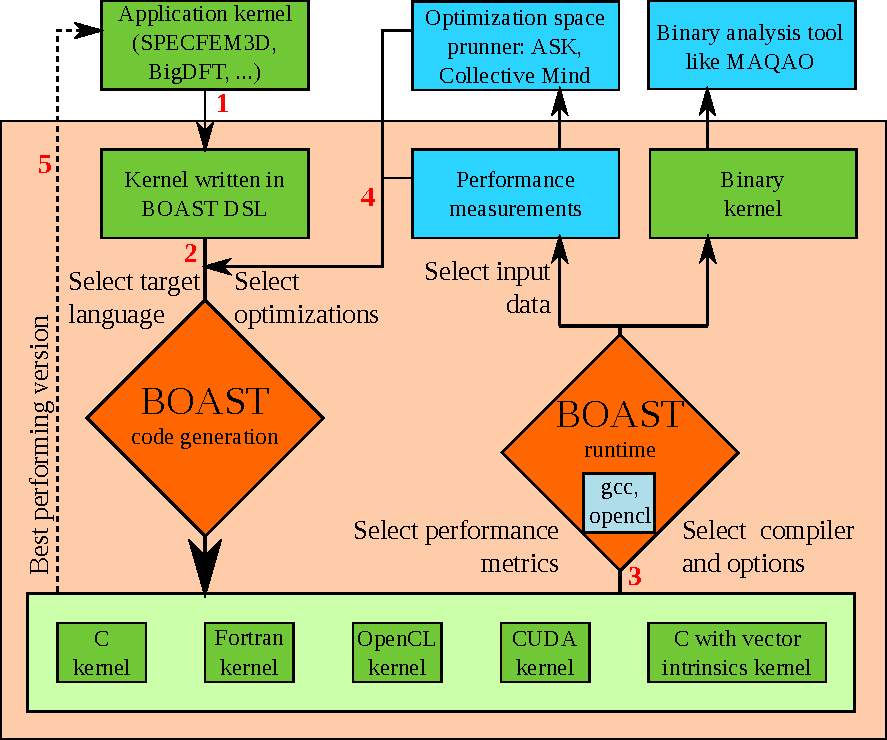
\includegraphics[width=\textwidth]{BOAST_Workflow.pdf}
\caption{Structure and Work-flow of the BOAST framework.}
\label{fig:boast_workflow}
\end{center}
\end{figure}

BOAST provides scientific application developers with a framework to develop and
test application computing kernels~\cite{videau2013boast}.
Figure~\ref{fig:boast_workflow} illustrates the envisioned work-flow and program
structure.
The user starts from an application kernel (either designed or implemented), and
write it in a dedicated language (step 1).
The language provides enough flexibility for
the kernel to be meta-programmed with several orthogonal optimizations. Then the
developer selects a kernel configuration and a target language. Those
parameters define the output source code that will be generated by BOAST (step
2). The resulting code source is then built according to the user specified
compiler and options (step 3). If input data are available then the kernel can
be benchmarked and tested for non regression. Based on the results, other
optimizations can be selected (step 4) or new optimizations can be added to the
BOAST sources. The process can be repeated until a good candidate is found on
the target platform. The resulting kernel is then added to the program (step 5).

Several steps in the work-flow can be automated: optimization and compiler flags
exploration, non regression testing, benchmarking... This automation can be
scripted by the user or by interfacing other dedicated tools. In order
to achieve those goals three aspects should be considered:
\begin{itemize}
\item code description,
\item code generation,
\item and kernel execution run-time.
\end{itemize}


  \subsection{Kernel Description Language}


%  \begin{itemize}
%  \item Abstraction of programming concepts: variables, procedures (
%portability, productivity )
%  \item Operator overloading: simpler syntax ( productivity, portability )
%  \item Two languages in one ( productivity, performance ) 
%  \end{itemize}

Usually computing kernels are hotspots of an HPC application, and they are most
of the time based on a loop nest. A lot of efforts are dedicated to their tuning
and the obtained result is often quite different from the original procedure.
Several transformations can be applied to such kernels. And those optimizations
are often applied manually as compiler may fail to recognise the opportunity.

There are many different loop optimization techniques~\cite{wolf1991loop}. We
can cite loop skewing~\cite{wolfe1986loops} (derives nested loops wavefronts)
or loop interchange~\cite{allen1984automatic} (loop variables change places).

The importance of  correct loop imbrication on BLAS~\cite{lawson1979basic}
operations is studied in~\cite{soliman2009performance}, and shows performance
increase of a factor up to 5 when using correct loop imbrication. The importance
of code transformation is stressed in~\cite{ye2011porting}, where a selection of GPU
kernels are ported to CPU and optimized.

BOAST kernel description language should be able to express all these
optimizations. This gives us a set of constraints to implement in the language:
\begin{itemize}
\item Arbitrary number of variables have to be created and manipulated (types,
attributes...).
\item Procedures have to be abstracted (reunite Fortran and C like languages,
attributes...).
\item Functions must be available.
\item Variables, constants and functions must be composed in complex
Expressions.
\item Basic control structures (for, while, if/else...) have to be abstracted.
\item Powerful array management (several dimensions, transformations,
indexing...).
\end{itemize}

%\begin{figure}
%\begin{center}
%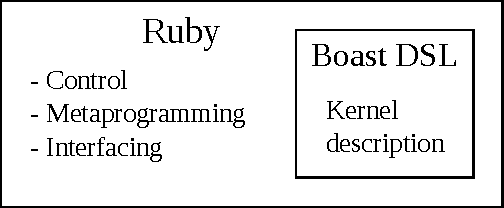
\includegraphics[scale=0.8]{BOAST_DSL.pdf}
%\caption{BOAST DSL intent.}
%\label{fig:dsl}
%\end{center}
%\end{figure}

In order to manipulate those abstractions we want to have a syntax resembling
what programmers use. For instance, commonly used operators have to be available
and behave as expected. It must also be possible to differentiate an action on
an abstraction in the context of an expression and in the context of the
management of this expression. $c = a + b$, an expression that affects the
results of $a + b$ to $c$  is not equal to $c \leftarrow a + b$, which saves the
expression $a + b$ to a variable $c$. This is why an embedded domain specific
language approach was selected~\cite{hudak1996building}. This allows for the
coexistence of two languages: the host language and the Domain Specific Language (DSL).
In our case, DSL allows the description of the kernel ($c = a + b$) while the host language
provides the meta programming of the kernel ($c \leftarrow a + b$)%, cf Figure~\ref{fig:dsl}
. Operator overloading of the host language will provide the familiar syntax
programmers are accustomed to. The host language will also provide easy
interfacing with libraries we might need during the development of our framework.

It was also important to have our constructs like \emph{for} loops to have a
syntax approaching those commonly found in programming languages. To this end, we
needed a language which could seamlessly pass a block of code to a function.
Ruby~\cite{matsumoto2002ruby} is one such language. It has deep introspection
capabilities as well. This is the main reason why it was selected.

    \subsubsection{BOAST Keywords}

In order to clearly differentiate what is going to be generated from what is
related to manipulations in the host language four keywords were defined. They
are \emph{decl}, \emph{pr}, \emph{opn} and \emph{close}. As the language is an
EDSL, these four keywords are methods in the BOAST namespace. Sample usage of
these keywords will be found in the next Figures.
%Usage of these keywords can be found on Figure~\ref{fig:keywords}.

The \emph{decl} method is used to declare variables or procedures and functions.

The \emph{pr} method calls the public \emph{pr} method of Objects it is
called on. Each BOAST object is responsible for printing itself correctly
depending on the BOAST configuration at the time the print public method is
called. Calling directly the print method of a BOAST object yields the same
result.

The \emph{opn} method can be used to print the beginning of a control
structure without an associated code block.

The \emph{close} method is the counterpart to the \emph{opn} method. It is used
to close a control structure without an associated code block.

    \subsubsection{BOAST Abstractions}

BOAST defines several classes that are used to represent the structure of the
code. These classes can be sorted in two groups, algebraic related and control
flow related:

      \paragraph{Algebra}

\begin{figure}
\lstset{style=BOAST,
        caption={BOAST code}, 
        label={lst:BOAST_algebra},
        numbers=left }
\begin{lstlisting}
i = BOAST::Int("i") # or BOAST::Variable::new("i", Int)
k = BOAST::Int("k", :size => 8)
l = BOAST::Real("l", :dim => [ BOAST::Dim(-5, 21) ], :local => true )
BOAST::decl i, k, l
BOAST::pr i === 5
j = i + 5
BOAST::pr k === j * 2
BOAST::pr l[k] === 1.0
BOAST::register_funccall("sin")
BOAST::pr l[k+1] === BOAST::sin(j)
\end{lstlisting}

\begin{minipage}[b]{0.50\linewidth}
\centering
\lstset{style=customf,
        caption={Fortran output.},
        label={lst:BOAST_algebra_FORTRAN} }

\begin{lstlisting}
integer(kind=4) :: i
integer(kind=8) :: k
real(kind=8), dimension(-5:21) :: l
i = 5
k = (i + 5) * (2)
l(k) = 1.0_wp
l(k + 1) = sin(i + 5)
\end{lstlisting}
\end{minipage}
\hspace{0.04\linewidth}
\begin{minipage}[b]{0.44\linewidth}
\centering
\lstset{style=customc,
        caption={C output.},
        label={lst:BOAST_algebra_C} }

\begin{lstlisting}
int32_t i;
int64_t k;
double l[27];
i = 5;
k = (i + 5) * (2);
l[k - (-5)] = 1.0;
l[k + 1 - (-5)] = sin(i + 5);
\end{lstlisting}
\end{minipage}
\caption{BOAST Code Snippet for Variables and Expressions}
\label{fig:BOAST_algebra}
\end{figure}
The first and most fundamental abstraction is named Variable. Variables have a
type, a name and a set of named attributes. The existing attributes are mainly
inspired from Fortran. Those attributes are not limited and can be arbitrarily
enriched, allowing a lot of flexibility in Variable management.

The second abstraction is named Expression. It combines variables into
algebraic or logic expressions. Most of the classical operators are overloaded
for those two abstractions and thus the syntax of the expressions are rather
straightforward. The exception is the assignment operator as it is important to
differentiate between assigning an Expression or a Variable in the Ruby context
and the assignment operator in the context of a BOAST Expression. Thus the
assignment in a BOAST Expression is represented as the \emph{===} operator,
while the classical assignment is kept as the \emph{=} operator. Function calls
(FuncCall) are also abstracted and can be used in Expressions.

Figure~\ref{fig:BOAST_algebra} shows some basic usage of both Variables and
Expressions as well as the \emph{pr} and \emph{decl} keywords. For clarity we
stayed out of BOAST namespace so BOAST related class and methods are prefixed
with \emph{BOAST::}. Listing~\ref{lst:BOAST_algebra} shows the BOAST code that
produces the Fortran (Listing~\ref{lst:BOAST_algebra_FORTRAN}) and C
(Listing~\ref{lst:BOAST_algebra_C}) output. At first we define 2 Variables
\emph{i} and \emph{k} (note that \emph{k} is $64$ bit integer). The third
variable named \emph{l} is a one dimensional local array of length $27$, it
is indexed in the range $-5$ to $21$. All those Variables are affected to Ruby
variables of the corresponding name.

On Line~4 we declare those three variables. Variable \emph{i} is then affected
the value 5. On Line~6 the \emph{j} Ruby variable is used to store the BOAST
expression \emph{$i+5$}. This variable will the be used transparently through
the rest of the program.

On Line~8 we use the \emph{k} variable to index into the array \emph{l} using
the bracket operator. Would the array be multidimensional the index would be
comma separated, similar to Fortran notation.

On the last line, a call to the \emph{sin} function is made through the creation
of a FuncCall object.  The possibility to use this method is declared using the
\emph{register\_funccall} method.

      \paragraph{Control Structures}

\begin{figure}
\lstset{style=BOAST,
        caption={BOAST code}, 
        label={lst:BOAST_control},
        numbers=left }
\begin{lstlisting}
BOAST::register_funccall("modulo")
i = BOAST::Int("i")
j = BOAST::Int("j")
BOAST::pr j === 0
BOAST::pr BOAST::For( i, 0, 100 ) {
  BOAST::pr BOAST::If( BOAST::modulo(i,7) == 0 ) {
    BOAST::pr j === j + 1
  }
}
\end{lstlisting}

\begin{minipage}[b]{0.47\linewidth}
\centering
\lstset{style=customf,
        caption={Fortran output.},
        label={lst:BOAST_control_FORTRAN} }

\begin{lstlisting}
j = 0
do i = 0, 100, 1
  if (modulo(i, 7) == 0) then
    j = j + 1
  end if
end do
\end{lstlisting}
\end{minipage}
\hspace{0.04\linewidth}
\begin{minipage}[b]{0.47\linewidth}
\centering
\lstset{style=customc,
        caption={C output.},
        label={lst:BOAST_control_C} }

\begin{lstlisting}
j = 0;
for (i = 0; i <= 100; i += 1) {
  if (modulo(i, 7) == 0) {
    j = j + 1;
  }
}
\end{lstlisting}
\end{minipage}
\caption{BOAST Code Snippet for control structures}
\label{fig:BOAST_control}
\end{figure}

The classical control structures are implemented. \emph{If}, \emph{For},
\emph{While}, \emph{Case} are abstractions in BOAST matching the behavior of
corresponding control structures in other languages. An exception is the For in
BOAST more closely matches the for in Fortran than the one in C.

Figure~\ref{fig:BOAST_control} shows some basic usages of the control structures.
The example shows a C macro or function that behaves similarly to the Fortran modulo
intrinsic. The sample script (inefficiently) computes and stores in \emph{j} the
number of multiples of $7$ in the 0 to 100 range. It uses the For and If control
structures. A Ruby block is passed to each of those constructs. This block is
evaluated at the time the construct is printed. If several such constructs are
needed (in an \emph{if elsif else} case, for instance) they can be explicitly
passed as parameters using the \emph{lambda} Ruby keyword.

\begin{figure}
\lstset{style=BOAST,
        caption={BOAST code}, 
        label={lst:BOAST_procedure},
        numbers=left }
\begin{lstlisting}
n = Int("n", :dir => :in)
ndat = Int("ndat", :dir => :in)
x = Real("x", :dir => :in, :dim => [ Dim(0, n-1), Dim(ndat) ])
y = Real("y", :dir => :out, :dim => [ Dim(ndat), Dim(0, n-1) ])
p = Procedure("magicfilter", [n, ndat, x, y])
opn p
close p
\end{lstlisting}

\lstset{style=customf,
        caption={Fortran output.},
        label={lst:BOAST_procedure_FORTRAN} }

\begin{lstlisting}
SUBROUTINE magicfilter(n, ndat, x, y)
  integer(kind=4), intent(in) :: n
  integer(kind=4), intent(in) :: ndat
  real(kind=8), intent(in), dimension(0:n - (1), ndat) :: x
  real(kind=8), intent(out), dimension(ndat, 0:n - (1)) :: y
END SUBROUTINE magicfilter
\end{lstlisting}
\lstset{style=customc,
        caption={C output.},
        label={lst:BOAST_procedure_C} }

\begin{lstlisting}
void magicfilter(const int32_t n, const int32_t ndat,
                 const double * x, double * y) {
}
\end{lstlisting}
\caption{BOAST Code Snippet for Procedure}
\label{fig:BOAST_procedure}
\end{figure}

The last control structure is Procedure. It describes either procedures
or functions. Figure~\ref{fig:BOAST_procedure} presents the use of this
abstraction. It illustrates the signature of a real kernel from BigDFT. This kernel uses
an input array \emph{x} and an output array \emph{y} of double precision
numbers. Those arrays have two dimensions which depend on input variables
\emph{n} and \emph{ndat}. We can see here the use of the \emph{opn} and
\emph{close} keywords that are used to print a control structure without an
associated Ruby block. This time we placed ourselves inside of BOAST namespace.

The generated outputs in Fortran (Listing~\ref{lst:BOAST_procedure_FORTRAN}) and
C (Listing~\ref{lst:BOAST_procedure_C}) show the difference in meta-information that is
kept between both versions.
  
%Considering source-to-source transformations that we investigate with the BOAST
%tool in this paper, we can compare ourselves to POET~\cite{POET2012}  and
%ABCLibScript~\cite{ABCLib2006}. However, both tools apply transformations
%to the syntaxic tree of a program while BOAST intervenes well before in the
%transformation process. Indeed, one may first use BOAST on order to generate a
%program (a specific syntactic tree) and then benefit from the transformation
%facilities offered by one of the above tools.

\subsection{BOAST Run-time}

In the previous Section we presented BOAST's language. This allows us to
describe procedures and functions and to meta-program them using Ruby.
Each version has to be compiled, linked and executed to assess its performance
in order to find the best version of a computing kernel.  This can be very
time consuming if this process cannot be automated. By enabling more versions
for evaluation, the automation will bring improved portability, better performance,
and in the end will improve the productivity of the developer.

In this section we will present the different aspects of BOAST run-time that
allow this automation. Those aspects include:
  \begin{itemize}
  \item multi target language generation ( performance, portability )
  \item compilation ( productivity, performance )
  \item execution ( productivity, performance )
  \item tracer, dumper and replay for non regression tests ( productivity )
  \end{itemize}

  \subsubsection{Multi-target Language Generation}
\label{sec:multitarget}
Language availability and performance varies between platforms. It is thus
important to express computing kernels in different languages, based
on the availability and their respective merits on the target platform. Some
languages have additional features, such as languages that target GPUs
(OpenCL, CUDA). The developer should be given tools to determine what kind of
language is currently used in order to be able to use those additional features.

Similarly the target language must be changed with ease in order to compare
different alternatives. Two methods are dedicated to this task: \emph{set\_lang}
and \emph{get\_lang}. The target language can also be set through an environment
variable before launching BOAST, allowing for easy command line scripting.

  \subsubsection{Compilation}

Compilation of the generated kernels must also be very flexible because HPC
application developers may encounter platforms with very diverse compilation environments.
Proprietary and dedicated compilers are common on HPC infrastructures. Thus
BOAST build system exhibits similar behavior to common build systems. Compilers
and their compile/build options can be specified at several
places. The list by increasing order of precedence includes: BOAST configuration
file, environment variables, and at kernel build time.

This way the framework to test different compiler optimizations is completely
available and performance study can include both kernel related parameters and
compilation related parameters. This behavior is contained in the \emph{CKernel}
class of BOAST. When instantiating this class a BOAST \emph{Procedure}
representing the entry point of the kernel is specified.

  \subsubsection{Execution}

The next logical step is to benchmark the built kernel. BOAST offers a simple
way to run a kernel that was successfully built while staying within BOAST.
A built BOAST \emph{CKernel} exposes a run method that accepts arguments corresponding
to the BOAST \emph{Procedure} used to instantiate the kernel. Arrays must be
instances of \emph{NArray} which are numerical arrays that use C arrays
underneath.

Arrays which correspond to output parameters will be modified during the
execution of the kernel so results can be checked. This allows for easy non
regression testing. The run method also returns information (and result for
kernels that are functions as well as output scalars) about the run. For
instance, one such information includes the run time of the kernel and it is
obtained using the system-wide real-time clock. Other probes can be inserted
at compile-time, if needed.
BOAST also supports PAPI~\cite{mucci1999papi} to capture hardware performance 
counters during each kernel execution.

  \subsubsection{Kernel Replay}

The non regression methodology presented before is viable provided input data
can be generated at run-time. For instance, in the case of the Laplace kernel,
generating an input image and the corresponding reference output image, using a
reference implementation, is easy. Unfortunately it is not always possible, some
applications have complex data patterns that are difficult to
synthesize without running the full application. Thus BOAST offers a way to load
binary data from the file system and use them as inputs of a kernel. Outputs can
also be checked against those binary data thus enabling (almost) data oblivious
non regression testing.

In order to use this methodology one has to be able to trace an application to
get input data. Such a tracer, dedicated to CUDA and OpenCL, will be presented
in the next subsection.

\subsection{Non Regression Testing Using Trace Debugging}
\label{sec:gputrace}

Debugging applications running on GPU environments is well-recognized as a hard
and time-consuming activity. In complement with BOAST, we designed a trace-based
debugging tool that simplifies this porting operation. The tool relies on BOAST
support of multi-target code generation (Section~\ref{sec:multitarget}), used to
validate an application from one GPU-programming framework to another or between
different implementations using the same programming model. A case-study of the
port of a CUDA application to OpenCL is presented in
Section~\ref{subsec:specfem}.

The idea behind the tool is based on the assumption that the different GPU
ports of the code should do the very same operations, at least at the logical
level (the APIs will have \emph{implementation} differences, but they should
offer nonetheless same functionalities). The usage of BOAST framework sustains
this assumption, as both sets of kernels should be generated from the same
source code.

Hence, the verification and validation of the new port can be
narrowed down to asserting that both codes apply the same operations
on the GPU. And the debugging part will consist in understanding what
diverges. To that purpose, we developed \code{GPUTrace}, inspired by
\code{strace} and \code{ltrace} tools: \code{GPUTrace} dynamically
preloads a library between the application and the GPU library, and
collects the function name, execution range and argument values (input
\emph{and} output) of the relevant function calls. These information
are traced in a unified format for all the APIs. This is a custom
trace format. Listing~\ref{lst:GPUTrace} presents a sample output
generated during \Specfem tracing.

However, in contrast with \code{strace} and \code{ltrace},
\code{GPUTrace} has to be \emph{state-full}. Indeed, most of API
parameters are handles to opaque types. So, in order to generate
meaningful traces, \code{GPUTrace} gathers information about these
objects at creation time (handle value, buffer creation size and
attributes, kernel name and prototype, \etc{}) and re-injects this
information when the objects used. A state-less implementation of
\code{GPUTrace} would highly rely on the GPU libraries introspection
capabilities, which seem not possible at the moment.

\lstset{style=customgputrace,
        caption={GPUTrace sample trace}, 
        label={lst:GPUTrace},
        numbers=left}
\begin{lstlisting}
New kernel: update_potential_kernel
...
New buffer #94, 2Mb, READ_WRITE (0x74d0420)
New buffer #95, 2Mb, READ_WRITE (0x74d08d0)
New buffer #96, 2Mb, READ_WRITE (0x74d0d80)
...
Buffer #94 written, 2314764b at +0b 
Buffer #95 written, 2314764b at +0b
Buffer #96 written, 2314764b at +0b
...
update_disp_veloc_kernel<128,1><4522,1>(
     float *displ=<buffer #94 1.00e-24, 1.00e-24, 1.00e-24, 1.00e-24, ...>
     float *veloc=<buffer #95 0.00e+00, 0.00e+00, 0.00e+00, 0.00e+00, ...>
     float *accel=<buffer #96 0.00e+00, 0.00e+00, 0.00e+00, 0.00e+00, ...>
     const int size=<578691>
     const float deltat=<1.365914e-04>
     const float deltatsqover2=<9.328606e-09>
     const float deltatover2=<6.829570e-05>
     ----
     <out> float *displ=<buffer #94 1.000e-24, 1.00e-24, 1.00e-24, 1.00e-24, ...>
     <out> float *veloc=<buffer #95 0.000e+00, 0.00e+00, 0.00e+00, 0.00e+00, ...>
     <out> float *accel=<buffer #96 0.000e+00, 0.00e+00, 0.00e+00, 0.00e+00, ...>
);
\end{lstlisting}

Once two call traces have been generated by \code{GPUTrace}, the user
can compare them with a graphical \code{diff} tool, and spot the
different porting mistakes: two parameters reversed, an offset
incorrectly applied, \etc{}

By default, \code{GPUTrace} only prints a unique identifier (the
creation index) for the memory buffers.  Additionally, \code{GPUTrace}
supports several modifier flags. One flag can be activated
to append the first bits of the buffer to the trace, printed in the
right format, for visual inspection. Another flag can be set to
dump the whole content of the buffer into a file, for a full
inspection.

This last option is also useful for generating \emph{replay buffers}
for BOAST kernel execution. With a set of filters based on kernel
names and execution counters, developers can precisely select which
kernel execution parameters should be dumped, for further reuse as
real-case benchmarks and non-regression testing.

\section{BOAST Use Cases}
\label{use_cases}

In this section we will present the benefits of using BOAST on the Laplace
motivating example as well as two scientific applications that use BOAST. The
first one, BigDFT~\cite{genovese2008daubechies}, uses BOAST in order to develop new
functionalities with performance portability in mind. The second one,
SPECFEM3D~\cite{komatitsch2011fluid}, uses BOAST to factorize OpenCL and CUDA
development, while having robust non regression tests.

  \subsection{Laplace Filter Kernel}

Section~\ref{sec:laplace} presented the Laplace motivating example. From this
section we know that a number of optimizations can have an impact on the
performance of the kernel on the Mali architecture. But, what is the impact in other
architectures? And, are there additional optimizations that can impact the
performance?

    \subsubsection{Optimization Space}

The list of already identified optimizations are:
\begin{itemize}
\item vectorization,
\item intermediary data type,
\item number of pixels processed,
\item and synthesizing loads.
\end{itemize}
To create our generic implementation we decided to work at the component level
rather than the pixel level. This approach leads to more flexibility and
genericity when applying optimizations. We also decided to study the impact of
another parameter which is the number of components to process on the column
direction. This leads to being able to process tiles instead of only rows.

Here are the parameters we finally selected for our kernel optimization and
their possible values:
\begin{itemize}
\item \textit{x\_component\_number}: a positive integer
\item \textit{y\_component\_number}: a positive integer
\item \textit{vector\_length}: 1, 2, 4, 8 or 16
\item \textit{temporary\_size}: 2 or 4
\item \textit{synthesize\_loads}: \textit{true} or \textit{false}
\item \textit{vector\_recompute}: \textit{true} or \textit{false}
\end{itemize}
The last parameter is used when \textit{x\_component\_number} is not divisible by
\textit{vector\_length}. Two solutions are possible then, divide the remainder
of the division in vectors of smaller sizes (\textit{vector\_recompute} =
\textit{false}) or load more data and compute useless values in vectors of the
specified size (\textit{vector\_recompute} = \textit{true}).
This last option mimics the behavior of the ARM implementation, although when
working at the component level it may not be a valuable thing to try.

    \subsubsection{Performance Results}

Table~\ref{tbl:ARM} show the best results obtained by ARM on different images
compared to the naive implementation and to the best version version BOAST
found. It shows that the generated version systematically outperforms the hand
optimized version. As far as the optimization options are concerned, the results
are disappointing: the same kernel configuration is the best for all image
sizes. This kernel uses \textit{x\_component\_number} = 16,
\textit{y\_component\_number} = 1, \textit{vector\_length} = 16,
\textit{temporary\_size} = 2 and \textit{synthesize\_loads} = false.
\textit{vector\_recompute} because \textit{x\_component\_number}
== \textit{vector\_length}. Those results show that, when working on full
vectors, synthesizing the loads is harmful to performance and the programmer is
better of trusting the cache to load each vector in one cycle without
compromising the bandwidth. The results shown here are the best of four runs for
each configuration.

\begin{table}
\centering
\begin{tabular}{|l|r|r|r|r|r|}
\hline
Image Size  & Naive (s) & Best (s) & Acceleration & BOAST (s) & Acceleration \\
\hline
768 x 432   & 0.0107    & 0.00669  & x1.6         & 0.000639  & x16.7 \\
\hline
2560 x 1600 & 0.0850    & 0.0137   & x6.2         & 0.00687   & x12.4 \\
\hline
2048 x 2048 & 0.0865    & 0.0149   & x5.8         & 0.00715   & x12.1 \\
\hline
5760 x 3240 & 0.382     & 0.0449   & x8.5         & 0.0325    & x11.8 \\
\hline
7680 x 4320 & 0.680     & 0.0747   & x9.1         & 0.0581    & x11.7 \\
\hline
\end{tabular}
\caption{Best performance of ARM Laplace kernel.}
\label{tbl:ARM}
\end{table}

But what if we run our benchmark on other architectures? Table~\ref{tbl:other}
shows the results obtained when running our BOAST implementation on other
architectures. The chosen architectures include an Intel i7-2760QM CPU (Sandy
Bridge architecture) that supports OpenCL 1.2 and a system with an NVIDIA gtx680 GPU that
supports OpenCL 1.1. We see that the performance ratio between the different
architectures is stable across image sizes.

The optimization parameters selected are not the same for those architectures.
Indeed, the Intel CPU favors kernels that have the parameters:
\textit{x\_component\_number} = 16,
\textit{vector\_length} = 8,
\textit{temporary\_size} = 2 and \textit{synthesize\_loads} = false. Once again
\textit{vector\_recompute} does not apply. \textit{y\_component\_number} varies
from 4 to 2 when image size increase, thus decreasing task granularity as the
global work size increase. This result is unexpected and understanding why this
happen could be interesting. The NVIDIA GPU favors processing square tiles:
\textit{x\_component\_number} = 4, \textit{y\_component\_number} = 4,
\textit{vector\_length} = 4, \textit{temporary\_size} = 2 and
\textit{synthesize\_loads} = false. Once more, \textit{vector\_recompute} has no 
meaning.

\begin{table}
\centering
\begin{tabular}{|l|r|r|r|r|r|}
\hline
Image Size & BOAST ARM (s) & BOAST Intel & Ratio & BOAST NVIDIA & Ratio \\
\hline
768 x 432   & 0.000639     & 0.000222    & x2.9  & 0.0000715    & x8.9  \\
\hline
2560 x 1600 & 0.00687      & 0.00222     & x3.1  & 0.000782     & x8.8  \\
\hline
2048 x 2048 & 0.00715      & 0.00226     & x3.2  & 0.000799     & x8.9  \\
\hline
5760 x 3240 & 0.0325       & 0.0108      & x3.0  & 0.00351      & x9.3  \\
\hline
7680 x 4320 & 0.0581       & 0.0192      & x3.0  & 0.00623      & x9.3  \\
\hline
\end{tabular}
\caption{Best performance of Laplace Kernel on several architectures.}
\label{tbl:other}
\end{table}

    \subsubsection{Laplace Conclusion}

In this Subsection we have shown the interest of BOAST in optimizing a well-known
algorithm across different architectures. Chosen optimization combinations
are highly dependent on the targeted architecture. In the next Subsections we
will show that our methodology also applies to real applications.

  \subsection{Creating an Auto-Tuned Convolution Library for BigDFT using
BOAST}

In 2005, the EU FP6-STREP-NEST BigDFT~\cite{genovese2008daubechies} project
funded a consortium of four European laboratories (L\_Sim - CEA Grenoble, Basel
University - Switzerland, Louvain-la-Neuve University - Belgium and Kiel
University - Germany), with the aim of developing a novel approach for DFT
calculations based on Daubechies wavelets.  Rather than simply building a DFT
code from scratch, the objective of this three-years project was to test the
potential benefit of a new formalism in the context of electronic structure
calculations.

As a matter of fact, Daubechies wavelets exhibit a set of properties which make
them ideal for a precise and optimized DFT approach. In particular, their
systematicity allows to provide a reliable basis set for high-precision
results, whereas their locality (both in real and reciprocal space) is highly
desired to improve the efficiency and the flexibility of the processing. Indeed,
a localized basis set allows to optimize the number of degrees of freedom for a
required accuracy~\cite{genovese2008daubechies}, which is highly desirable given
the complexity and inhomogeneity of the systems under investigation nowadays.

Despite the application is mainly written in Fortran, it currently includes
360 kLOC and 70kLOC of Fortran and C languages, respectively, accounting for more
than 50\% of the code base.  It is a parallel application
based on the standards MPI~\cite{mpi} and OpenMP~\cite{openmp}.  It also
supports CUDA~\cite{cuda} and OpenCL~\cite{opencl}.  In the recent years this
code has been used for many scientific applications, and its development and
user consortium is continuously growing.  Massively parallel computations are
routinely executed with the BigDFT code, either in homogeneous or hybrid
architectures.  In 2009, the French Bull-Fourier award was attributed for the
implementation of the hybrid version of BigDFT~\cite{genovese2009density}.

%As it is used on systems that may
%have very different architectures, it is of great importance to be able to
%optimize and run the application according to the specific underlying platform.

    \subsubsection{BigDFT}

In the Kohn-Sham (KS) formulation of DFT, the electrons are associated to
wavefunctions (orbitals), which are represented arrays of floating point
numbers. In wavelets formalism, the operators are written via convolutions with
short, separable filters.  The detailed description of how these operations are
defined is beyond the scope of this report and can be found in the BigDFT
reference paper~\cite{genovese2008daubechies}.

% Convolutions are among the basic processing blocks of BigDFT. Special care
% has to be taken regarding their performances. 
The CPU convolutions of BigDFT have thus been thoroughly optimized.  In a recent
paper~\cite{videau2013optimizing}, the optimization of the CPU convolutions of
BigDFT has been extensively considered.
%BigDFT is characterized by its extensive use of convolution
%operators~\cite{nussbaumer1982fast} applied on large arrays of data.  
One example of a specific convolution, called
MagicFilter~\cite{Genovese|CAS2010}, can be seen in
Listing~\ref{lst:conv_example}.  It applies a filter $filt$ to the data set
$in$ and then stores the result in the data set $out$ with a
transposition~\cite{Goedecker1993}.

\lstset{	language=C, 
		basicstyle=\scriptsize, 
		backgroundcolor=\color{white}, 
		frame=single, 
		captionpos=b,
		caption={MagicFilter.}, 
		label={lst:conv_example}}
		
\begin{lstlisting}
double filt[16] = {F0, F1, ... , F15};
void magicfilter(int n, int ndat, double* in, double* out){
  double temp;
  int m;
  for( j = 0; j < ndat; j++) {
    for( i = 0; i < n; i++) {
      temp = 0;
      for( k = 0; k < 16; k++) {
        m = (i-7+k)%n
        temp += in[m + j*n] * filt[k];
      }
      out [j + i*ndat] = temp ;
    } 
  }
} 
\end{lstlisting}

As we can see, there are three nested loops working on arrays whose sizes vary.
Various optimizations can be applied to this treatment and may focus on the
loop structure, as well as on the size of the data. 
%In this paper we focus on this particular convolution and explore different
%optimizations whose nature is presented in detail in the next section.

    \subsubsection{A Generic Convolution Library}

The number of convolution kernels needed in BigDFT has been continuously
growing in the recent years.  Various boundary conditions and functionalities
have been added, making the BigDFT more and more powerful in terms of
scientific applications.  However, the cost of the maintenance and of
development of the convolutions is always a delicate point to be considered
while including a new functionality.  The convolution patterns are usually
rather similar, leading to code duplication and difficulties in code
maintainability.

It appears therefore very interesting to benefit from an automatic tool to drive
the implementation and the generation of new convolutions.  This would lead to
an optimized code, adapted to different computing platforms, that is optimally
factorized.  In addition to this point, the help of such code generator is also
important to build \emph{new science}: the cost of implementing new
convolutions would become so little that other functionalities (for example,
the generalization of the BigDFT convolutions to Neumann boundary conditions
or the usage of wavelet-on-the-interval basis) can be added with limited
manpower.

For these reasons, a convolution library has been engineered with the help of
BOAST.  The detailed API of the library will be described elsewhere.  The
spirit is similar to BLAS-LAPACK API, where low-level operations are scheduled
and called from high-level operations. The basic blocks will be comprised of
unidimensional wavelet transforms and convolutions applied to multidimensional
arrays. Combining those blocks will yield multidimensional transforms.

Each of the building blocks of these convolution libraries is optimally tuned
by BOAST by choosing the sources providing the optimal kernel for the chosen
computing platform.  The sources of these kernels are then collected and
compiled to meet the API of the library.

A library written in this way might have an impact going largely beyond the
community of BigDFT developers.  Indeed, convolutions are basic operations of
lots of scientific application codes, like for example finite differences
approaches, which are universally used in computational physics.

The interest in having a robust and optimally tuned library in this scientific
field is therefore evident. Techniques are under investigation to provide also
fine-tuned binaries to the end-user rather than the code sources, such that
more aggressive inter procedural optimization can be performed. Indeed, BOAST
finds the optimal source code for a given kernel and compiler configuration but
one could imagine using binary optimizer to the compiled binaries. Those
optimizers could be coupled to BOAST and the output of the process would be the
final binary rather than the source code. This experience therefore would be a
first step toward the release of a tunable optimised convolution library
oriented to computational physics communities.


    \subsubsection{Performance report}

Several kernels have already been implemented in BOAST for the convolution
library. Figure~\ref{fig:synthesis} shows the performance of the wavelet
transform operation as a factor of the unrolling length of the outer loop, the
language used to implement it as well as the activation or not of the OpenMP
parallelization. Results are given as a speedup compared to the sequential hand
tuned implementation that can be found in BigDFT. These tests were run on the
Intel Xeon X5550 that was used to hand optimize the code.

\begin{figure}
\begin{center}
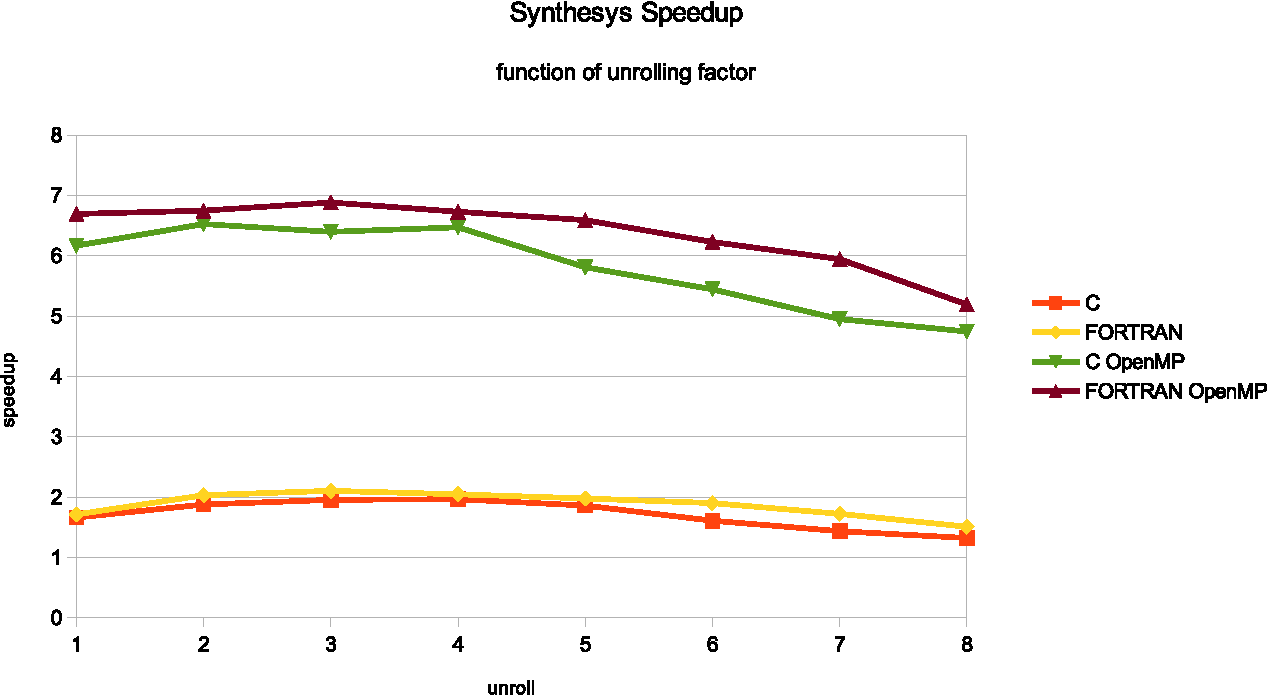
\includegraphics[scale=0.7]{Res_synthesis}
\end{center}
\caption{Impact of Unrolling, Language and OpenMP on a Wavelet Transform}
\label{fig:synthesis}
\end{figure}

We can see that this function is better optimized using Fortran and small
unrolling factors. In the hand optimized version the unrolling factor was chosen
much too high (a factor of 12 was used). This factor might have been optimal at
the time the procedure was optimized (compiler version changed in the meantime) but
since then the environment changed. Other optimizations have also been
incorporated in the BOAST sources, like the systematic inner loop unrolling, and
those could also help increase performance while limiting the interest of the
outer loop unrolling.

Nonetheless what is interesting from the physicist point of view is that the
generated source will give its better performance on a whole range of
architectures/compilers combinations than that of the hand tuned code.

%   BigDFT implementation of convolution/wavelets is a reference but is limited
%   in scope (1 wavelet family ands its derived operators).  Generalizing to
%   other wavelet families long and difficult if performance are to remain
%   good.
% 
% Idea: \begin{itemize} \item write a generic convolution library in BOAST
% \item BLAS like interface \item Provide a wide variety of building blocks
% \item Optimize thos blocks using BOAST \item Build either from source or
% directly link with binary \item Release complete library \end{itemize}
% 
% 
%   Characteristic use case driven
% 
%   Convolution Library: first step toward a dsl dedicated to wavelet
%   processing for Physics computing.
 


  \subsection{Porting SPECFEM3D to OpenCL using BOAST}
  \label{subsec:specfem}

In this last subsection, we study a free seismic wave propagation
simulator, \Specfem, in its \productname{Globe}
flavor\footnote{Specfem3d Globe --- CIG
  \url{http://www.geodynamics.org/cig/software/specfem3d-globe}}. \Specfem
simulates seismic wave propagation at the local or regional scale
based upon spectral-element method (SEM), with very good accuracy and
convergence properties. It is a reference application for super
computer benchmarking, thanks to its good scaling capabilities.


    \subsubsection{SPECFEM3D}

When we started to work on the project (version v2.1 of July 2013) it
supported graphics card GPU acceleration through NVidia \Cuda. This
GPU support came in addition to the MPI support implemented to enable
multi-CPU parallel computing. Most of \Specfem code-base is written in
\productname{Fortran2003}, only the GPU related parts are written in
C.  The split between CPU and GPU code was done at a rather fine
grain, as the application counted more than 40 GPU kernels. Some of
them were quite simple (\eg performing a few vector operations, but at
massively parallel scale), while at the other side of the spectrum,
some complex kernels took more than 80 parameters and perform very
specific physical transformations.

Because of the complexity of wave propagation (and of the application
architecture), it is hard to impossible to define unit tests. Hence,
the application is validated by the accuracy of the results it
produces, that is, the accuracy of seismograms of the simulated
earthquakes, in comparison with the actual ones. Non-regression
testing (after new developments) is also based on these seismograms,
with measurements of the relative error between two identical
simulations.

As part of the Mont-Blanc project, we had to port \Specfem to \OCL, so
that it could be used to benchmark Mont-Blanc HPC platforms.

\subsubsection{Porting to OpenCL}

\subparagraph{Porting kernels to BOAST} 

Nvidia \Cuda and \OCL are based on the same programming model: a
massively parallel accelerator running in disjoint, non addressable
memory environment. Thanks to that proximity, we have been able to carry
out most of the porting task with only a limited knowledge about
\Specfem internal physics.

This lack of \Specfem internal knowledge led us to be particularly
careful to the path we undertook for the port, as we would have
been unable to understand how and why the application was not
operating properly, if it was to fail.

Hence, our first milestone in the port was the translation of
\Specfem's \Cuda kernels into BOAST EDSL. This way, we could ask BOAST
framework to generate a CUDA version of the kernels, plug them back
into \Specfem and get (after fixing compile-time errors---prototypes
and naming mistakes mainly) a first set of \Specfem seismograms.

As we had expected, the seismograms were erroneous. But with the help
of shell scripts and BOAST framework ability to store and provide the
kernels' original source code, we built a set of \Specfem binaries
including only \emph{one} BOAST-generated kernel, with all others
reference-kernels. Running and validating all these binaries enabled
use to pinpoint the misbehaving kernels. We finished the debugging
with a side-by-side comparison that highlighted the coding mistakes.

\subparagraph{Porting run-time to \OCL} The second part of the port
consisted in the translation of the CPU-side of the application, from
\Cuda API to \OCL API. Most of the functions of the interfaces are
very similar, with only naming-convention and data-structure
distinctions. Hence, it was clear that automatic rewriting tools
(namely \code{sed} regexp and \code{emacs-lisp} functions) could be
useful. To give an idea of the cost of a \emph{manual} rewriting, we
can count (in \# of \OCL API function calls): 70 kernel ``function
calls'', 790 arguments to set, 230 memory transfers, 160 buffer
creations, and 270 releases.

Once the transformations were applied,
compilation errors fixed, and \OCL unsuccessful function calls solved,
the application managed to complete its execution and generate a first
set of seismograms. And again, as expected and feared, these
seismograms were not valid as their shape was completely different from the
reference ones.

As we had already validated BOAST-generated kernels (and trusted \Cuda and \OCL
versions to be semantically identical), we knew that the bugs were now in the
usage of the run-time, and we had to find a way to understand where \Specfem's
\Cuda version of the code diverged from its \OCL counterpart. To help us in
that purpose, we had a strong assumption: both versions of the code were
supposed to perform exactly the same operations, with the same ``logical''
parameters (the APIs have \emph{implementation} differences, for instance \OCL
has two memory transfer functions, \code{clEnqueueReadBuffer},
\code{clEnqueueWriteBuffer}, whereas \Cuda has only one, with a direction
parameter \code{cudaMemcpy(..., dir)}, but above that, it is the same
functionality).

Hence, our idea for locating the execution problems was to make sure
that both execution actually did the same thing. As the \OCL results
were invalid, we knew the executions would diverge at one or several
points.

\subparagraph{Debugging \OCL Execution: \code{GPUTrace}} 

With the help of \code{GPUTrace} (Section~\ref{sec:gputrace}), we
could confront \Cuda and \OCL execution traces with a graphical
\code{diff} tool, and spot the different porting mistakes: some
parameters reversed, offsets incorrectly applied, \etc{}. 

One last problem remained, clearly highlighted by the seismograms not
matching perfectly (they had a similar shape, but with a reduced
intensity). We added more verbosity to \code{GPUTrace} output: first
the initial bits of the GPU memory buffers, then their full
content. The drift was visible in the trace, but it was nonetheless
unclear where it started. We finally got it after hours of code review
of BOAST kernels and \OCL code. One kernel was
\emph{three}-dimensional, whereas the others were two-dimensional. But
for all of them, only two dimensions were passed, and one was
missing.
%As it was the same person who coded the \OCL port and the GPU
%tracer, this third dimension was forgotten in both codes.

\subparagraph{Evaluation} Our \OCL/BOAST port of \Specfem is now
merged in \Specfem's development tree and under test and extension by
different research teams. On a platform with two K40x GPUs and N Intel
Xeon processors, we measured similar results between the original
\Cuda version and our BOAST-\Cuda version. With the same set of
optimization flags, BOAST \Cuda and \OCL version reported similar
execution time spans. The best execution speed was achieved with \Cuda
version though (25\% higher than \OCL), as one optimization parameter
(\code{CUDA\_LAUNCH\_BOUND}) cannot be passed, to \OCL run-time, as of version
1.1. This parameter, in addition to specifying the work group size (which can
be done in \OCL), also constrains the number of work group that must run in
parallel on a multiprocessor. This value is set to 7 in \Cuda. This means that
the compiler must be very conservative on register usage in order to allow this
parallelism which allows better overlapping of communications end computations.
This functionality is not supported in \OCL.

By refactoring GPU kernel code in BOAST EDSL, the size of kernel code
shrank by a factor of 1.8 (from 7500 to less than 4000 LOC, partly
because of code duplication, also removing manually unrolled
loops). This is beneficial for \Specfem as it improves the readability
and maintainability of its source code.

We have also been able to enhance \Specfem's non-regression test-suite
by adding per-kernel non-regression tests. This was done with the help
of \code{GPUTrace}, that we used to capture all the input parameters
of a particular \emph{valid} kernel execution, as well as the output
values. Then, during the non-regression testing, BOAST framework
loads these buffer files, allocates GPU memory and initializes it through
\Cuda or \OCL run-time, and triggers the kernel execution. A comparison
of the output values (for instance against a maximal error level)
validates the non-regression.

In the same mindset, we provided \Specfem test-suite with kernel
performance evaluation mechanisms. These tests will help developers to
try new optimizations in kernel code and measure their impact, without
executing the whole application.

\section{Related Work}

Code generation and auto-tuning techniques are not new. Nonetheless, with recent
developments in hardware, and the HPC landscape being as diverse as it is now,
there is a renewed interest in the field. This related work Section is split in
three parts, focusing first on Auto-tuning frameworks. Tools that provide a DSL
to describe computing kernels will then be presented. Last, optimization space
pruners and their ties to auto-tuning will be introduced.

  \subsection{Application Auto-Tuning} 

  The most convenient way to obtain an application that can be auto-tuned on a
given platform is to base this application on a widely used computing library.
BLAS~\cite{dongarra1990set} and LAPACK~\cite{laug} are such libraries. These
libraries are either hand tuned for selected platforms or have auto-tuned
implementations. Atlas~\cite{whaley04} is an auto-tuned implementation of
BLAS/LAPACK. ATLAS authors defined the \emph{Automated Empirical Optimization of
Software} methodology that we implemented with BOAST. Their kernel generation is
done using macro-functions in C.

  Nonetheless many application formalisms cannot be reduced to standardized
library or border on what could be considered edge cases for those libraries and
not as optimized as more general cases. Orio~\cite{Hart2009:Orio} is an
auto-tuning framework that has an approach close of that of BOAST but they are
based on an annotated DSL describing loop transformation rather than a more
generic EDSL. Halide~\cite{ragan2013halide} is an auto-tuning framework
dedicated to image processing. It can also be used to describe other
operations on memory buffers. Those two frameworks propose automated search
space exploration to find the best version of a kernel.
LGen~\cite{spampinato2014basic} is a compiler that generates linear algebra
programs for small fixed size problems. Knowing the problem size it fully
unrolls and vectorizes loops, yielding better performance than state of the
art generic implementations.

  \subsection{Kernel Description DSL}

  The idea to describe computing kernels using a DSL has been already explored.
SPIRAL~\cite{puschel2004spiral} is a decade old generation
framework for signal processing. It uses a proprietary DSL, SPL (Signal
Processing Language), to describe a DSP algorithm. This DSL is then transformed
into efficient programs in high level languages like C or Fortran.
POET~\cite{yi2007poet} also uses a DSL to describe custom code transformations,
like loop unrolling, loop blocking and loop interchange. Those transformation
can be parametrized in order to tune the application. Orio~\cite{Hart2009:Orio}
can be compared to POET as it aims at describing possible code transformations
using a DSL. All those approaches are very different from our as they put the
emphasis on compilation techniques whereas BOAST relies on the user to express
the different optimizations.

  Halide~\cite{ragan2013halide} is closer in some ways to our approach as it
uses an embedded C++ DSL to describe image processing algorithm. This DSL allows
decoupling the algorithm description from its scheduling. Each pixel in the
resulting image has a completely defined dependency tree with regard to pixels
in the input image (and intermediary results). During generation, depending on
memory and computing cost, some values are recomputed rather than fetched from
memory. We used Halide to implement the \emph{magicfilter} of BigDFT, but
unfortunately results were 4 to 5 times slower than the one we obtained with
BOAST. We speculate that the three-dimensional nature of our convolutions, as
well as the filter length, can be considered edge cases in Halide and quite far
from the intended target.

  \subsection{Optimization Space Pruner}

  Once auto-tuning techniques are used, the parameter space explodes and the
systematic sampling rapidly becomes impossible to achieve. The cost of finding
the optimal kernel parameters and environment parameters (compiler flags, used
language, ...) is rapidly prohibitive. Dedicated frameworks have been developed
to address this problem. Adaptive Sampling Kit (ASK)~\cite{castro2013adaptive}
is one such tool. It reduces the number of samples needed by creating a model of
the performance and by minimizing the number of samples needed to find the
parameters of this model. Several models and sampling techniques are
implemented.

  Collective Mind~\cite{fursin:hal-01054763} proposes similar techniques to
solve the problem but also stores and the results and complete experimental
setups in databases for future reference and reproducibility. This database
approach also enables easy parallelization of the experimental process.
Collective Mind also proposes collections of flags for many available
compilers/versions easing the exploration process.

\section{Conclusion and Future Works}

In this report we presented the BOAST infrastructure as well as its
application to three use cases from the Mont-Blanc project. Results are
encouraging as BOAST proved to be a powerful and flexible tool that allowed
gains in performance and performance portability.

Future development will focus on three goals. Interfacing with binary analysis
tools like MAQAO~\cite{djoudi2005exploring} in order to build a feedback loop to
guide optimization. Interfacing with search space modellers/pruners in order to
optimize the search of the optimal version of a kernel. Continue working on
vector code. For instance producing a collection of small to medium useful
vector patterns (transposition, for instance) in BOAST could really help develop
vectorized version of our algorithm.



%\section*{References}

\bibliography{D5.5}

\section*{Annexes}

This section will present some simple examples to familiarize the user with
BOAST. More samples can be found with source code from the program in the git
repository: \url{https://github.com/Nanosim-LIG/boast}.

\subsection*{Installation}

BOAST is Ruby based, so Ruby needs to be installed on the machine.
Installation of boast can be done using the Ruby built-in package manager:
\textit{gem}. See Listing~\ref{lst:BOAST_install} for reference.

\lstset{style=custombash,
        caption={BOAST installation}, 
        label={lst:BOAST_install},
        numbers=left }
\begin{lstlisting}
sudo apt-get install ruby ruby-dev
gem install --user-install BOAST
\end{lstlisting}

\subsection*{Variable and Procedure Declaration}

The following samples are presented using \textit{irb} Ruby interactive
interpreter. It can be launched using the \textit{irb} command in a terminal.
Listing~\ref{lst:variable_declaration} shows the declaration of two variables
of different kind.

\lstset{style=BOAST,
        caption={Variable Declaration},
        label={lst:variable_declaration}}
\begin{lstlisting}
irb(main):001:0> require 'BOAST'
=> true
irb(main):002:0> a = BOAST::Int "a"
=> a
irb(main):003:0> b = BOAST::Real "b"
=> b
irb(main):004:0> BOAST::decl a, b
integer(kind=4) :: a
real(kind=8) :: b
=> [a, b]
\end{lstlisting}

Listing~\ref{lst:procedure_declaration} shows the declaration of a procedure
using the two previous variables as parameters. For clarity, \textit{irb} echoes have
been suppressed.

\lstset{style=BOAST,
        caption={Procedure Declaration},
        label={lst:procedure_declaration}}
\begin{lstlisting}
005:0> p = BOAST::Procedure( "test_proc", [a,b] )
006:0> BOAST::opn p
SUBROUTINE test_proc(a, b)
  integer, parameter :: wp=kind(1.0d0)
  integer(kind=4) :: a
  real(kind=8) :: b
007:0> BOAST::close p
END SUBROUTINE test_proc
\end{lstlisting}

\subsection*{Switching Language}

Listing~\ref{lst:switching_language} shows how to switch BOAST to C. Available
languages are \textit{FORTRAN}, \textit{C}, \textit{CUDA} and \textit{CL}.

\lstset{style=BOAST,
        caption={Switching Language},
        label={lst:switching_language}}
\begin{lstlisting}
008:0> BOAST::lang = BOAST::C
009:0> BOAST::opn p
void test_proc(int32_t a, double b){
010:0> BOAST::close p
}
\end{lstlisting}

\subsection*{Defining a Complete Procedure}

Listing~\ref{lst:complete_procedure} shows how to define a procedure and the
associated code. Note that here the parameters of the procedure have been
associated a direction: one, \textit{a}, is an input parameter while the other
is an output parameter.

\lstset{style=BOAST,
        caption={Complete Procedure},
        label={lst:complete_procedure}}
\begin{lstlisting}
011:0> BOAST::lang = BOAST::FORTRAN
012:0> a = BOAST::Real( "a", :dir => :in)
013:0> b = BOAST::Real( "b", :dir => :out)
014:0> p = BOAST::Procedure( "plus_two", [a,b] ) {
015:1*   BOAST::pr b === a + 2
016:1> }
017:0> BOAST::pr p
SUBROUTINE plus_two(a, b)
  integer, parameter :: wp=kind(1.0d0)
  real(kind=8), intent(in) :: a
  real(kind=8), intent(out) :: b
  b = a + 2
END SUBROUTINE plus_two
018:0> BOAST::lang = BOAST::C
019:0> BOAST::pr p
void plus_two(const double a, double * b){
  (*b) = a + 2;
}
\end{lstlisting}

\subsection*{Creating, Building and Running a Computing Kernel}

Listing~\ref{lst:computing_kernel} shows how to create a Computing kernel
(\textit{CKernel}) and build it. Once a computing kernel is instantiated the
output of BOAST will be redirected to the computing kernel source code. Line 4
sets the entry point of the computing kernel to the procedure we just defined.
By default compilation commands are not shown unless an error occurs. This
behavior can be changed by switching to verbose mode.

When running the kernel all the arguments have to be specified. Running a
kernel returns a hash table containing information about the procedure
execution. In this simple case two informations are returned, first the value
of the output parameter \textit{b} and second the time the kernel execution
took.

\lstset{style=BOAST,
        caption={Computing Kernel},
        breaklines=true,
        breakautoindent=false,
        label={lst:computing_kernel}}
\begin{lstlisting}
020:0> BOAST::lang = BOAST::FORTRAN
021:0> k = BOAST::CKernel::new
022:0> BOAST::pr p
023:0> k.procedure = p
024:0> puts k
SUBROUTINE plus_two(a, b)
  integer, parameter :: wp=kind(1.0d0)
  real(kind=8), intent(in) :: a
  real(kind=8), intent(out) :: b
  b = a + 2
END SUBROUTINE plus_two
025:0> k.build
026:0> BOAST::verbose = true
027:0> k.build
gcc -O2 -Wall -fPIC -I/usr/lib/x86_64-linux-gnu/ruby/2.1.0 -I/usr/include/ruby-2.1.0 -I/usr/include/ruby-2.1.0/x86_64-linux-gnu -I/usr/include/x86_64-linux-gnu/ruby-2.1.0 -I/var/lib/gems/2.1.0/gems/narray-0.6.1.1 -DHAVE_NARRAY_H -c -o /tmp/Mod_plus_two20150309_4611_5a129k.o /tmp/Mod_plus_two20150309_4611_5a129k.c
gfortran -O2 -Wall -fPIC -c -o /tmp/plus_two20150309-4611-5a129k.o /tmp/plus_two20150309-4611-5a129k.f90
gcc -shared -o /tmp/Mod_plus_two20150309_4611_5a129k.so /tmp/Mod_plus_two20150309_4611_5a129k.o /tmp/plus_two20150309-4611-5a129k.o -Wl,-Bsymbolic-functions -Wl,-z,relro -rdynamic -Wl,-export-dynamic -L/usr/lib -lruby-2.1 -lrt
028:0> r = k.run(5,0)
029:0> puts r
{:reference_return=>{:b=>7.0}, :duration=>5.84e-07}
\end{lstlisting}

\subsection*{Using Arrays in Procedures}

Most computing kernels don't work on scalar values but rather on arrays of
data. Listing~\ref{lst:arrays} shows how to use arrays in computing kernels.
In this case we place ourselves in BOAST namespace to reduce the syntax
overhead. Variables \textit{a} and \textit{b} are one-dimensional arrays of
size \textit{n}. Arrays in BOAST start at index 1 unless specified otherwise.
For instance \lstinline!Dim(0,n-1)! would have created a dimension starting at
0. Array bounds can also be negative and several dimensions can be specified
to obtain muti-dimensional arrays.
For self contained procedures/kernels one can use the shortcut written on
line~13 to create a CKernel object. As we are not specifying build options the
build command can also be omitted and will be automatically called when
running the kernel the first time. Lines~17 to 19 are used to check the result
of the kernel.

\lstset{style=BOAST,
        caption={Array Usage},
        label={lst:arrays}}
\begin{lstlisting}
001:0> require 'BOAST'
002:0> require 'narray'
003:0> include BOAST
004:0> n = Int(  "n", :dir => :in )
005:0> a = Real( "a", :dir => :in,  :dim => [Dim(n)] )
006:0> b = Real( "b", :dir => :out, :dim => [Dim(n)] )
007:0> p = Procedure( "plus_two", [n, a, b] ) {
008:1*   decl i = Int( "i" )
009:1>   pr For( i, 1, n ) {
010:2*     pr b[i] === a[i] + 2.0
011:2>   }
012:1> }
013:0> k = p.ckernel
014:0> input  = NArray.float(1024).random
015:0> output = NArray.float(1024)
016:0> k.run(input.length, input, output)
017:0> (output - input).each { |val|
018:1*   raise "Error!" if (val-2).abs > 1e-15
019:1> }
020:0> stats = k.run(input.length, input, output)
021:0> puts "Success, duration: #{stats[:duration]} s"
Success, duration: 3.79e-06 s
\end{lstlisting}

\subsection*{The Canonical Case: Vector Addition}

Listing~\ref{lst:vector_add_decl} shows the addition of two vectors in a third
one. Here BOAST is configured to have arrays starting at 0 and to use single
precision reals by default (Lines~5 and 6).  The kernel declaration is
encapsulated inside a method to avoid cluttering the global namespace. Line 15
the expression \lstinline!c[i] === a[i] + b[i]! is stored inside a variable
\textit{expr} for later use. Lines~16 to 23 show that the kernel differs
depending on the target language, in CUDA and OpenCL each thread will process
one element.

\lstset{style=BOAST,
        caption={Vector Addition Declaration},
        label={lst:vector_add_decl}}
\begin{lstlisting}
require 'narray'
require 'BOAST'
include BOAST

set_array_start(0)
set_default_real_size(4)

def vector_add
  n = Int("n",:dir => :in)
  a = Real("a",:dir => :in, :dim => [ Dim(n)] )
  b = Real("b",:dir => :in, :dim => [ Dim(n)] )
  c = Real("c",:dir => :out, :dim => [ Dim(n)] )
  p = Procedure("vector_add", [n,a,b,c]) {
    decl i = Int("i")
    expr = c[i] === a[i] + b[i]
    if (get_lang == CL or get_lang == CUDA) then
      pr i === get_global_id(0)
      pr expr
    else
      pr For(i,0,n-1) {
        pr expr
      }
    end
  }
  return p.ckernel
end
\end{lstlisting}

Listing~\ref{lst:vector_add_run} shows the a way to check the validity of the
previous kernel over the available range of languages. The options that are
passed to run are only relevant for GPU languages and are thus ignored in
Fortran and C (Line~16). Success is only printed if results are validated,
else an exception is raised (Lines~17 to 20).

\lstset{style=BOAST,
        caption={Vector Addition Test},
        label={lst:vector_add_run}}
\begin{lstlisting}
n = 1024*1024
a = NArray.sfloat(n).random
b = NArray.sfloat(n).random
c = NArray.sfloat(n)

epsilon = 10e-15

c_ref = a + b

[:FORTRAN, :C, :CL, :CUDA].each { |l|
  set_lang( BOAST.const_get(l)  )
  puts "#{l}:"
  k = vector_add
  puts k.print
  c.random!
  k.run(n, a, b, c, :global_work_size => [n,1,1], :local_work_size => [32,1,1])
  diff = (c_ref - c).abs
  diff.each { |elem|
    raise "Warning: residue too big: #{elem}" if elem > epsilon
  }
}
puts "Success!"
\end{lstlisting}

\end{document}

% vim: set spell ft=tex fo=aw2t expandtab sw=2 tw=100:
